\chapter{Antecedentes}

En este capítulo se expondrán los fundamentos teóricos y conceptuales necesarios en el desarrollo del proyecto. Se abordarán los conceptos principales características de las antenas, ya que por naturaleza un radiotelescopio es una antena. Además, se explicará el funcionamiento de los receptores heterodinos, principal componente utilizado en la digitalización y adquisición de señales de RF. Para finalmente, abordar el concepto de radiotelescopio, la importancia de la línea de Hidrógeno neutro y el proyecto CHARTS.\\

\section{Fundamentos de antenas}

Una antena es un dispositivo usualmente pasivo que convierte radiación electromagnética del ambiente en corriente eléctrica y viceversa, dependiendo para que se utilice, pueden ser utilizadas para recibir o transmitir señales. Un radiotelescopio son antenas receptoras. Suele ser fácil calcular las propiedades de una antena transmisora y medir las propiedades de una antena receptora. Afortunadamente, la mayor parte de las propiedades de una antena transmisora (como el patrón de radiación) son las mismas al usar esta misma antena como receptora, así como cualquier medición de una antena receptora puede ser aplicada a esta antena cuando es usada para la transmisión \cite{Ransom2016}.\\

\subsection{Patrón de radiación}

El patrón de radiación es una representación gráfica de las propiedades radiativas de una antena. Se define como el gráfico de potencia transmitida por la antena, evaluada sobre una esfera de radio constante. Por razones prácticas se estudian cortes del patrón de radiación. Estos cortes son las curvas tridimensionales del patrón que son contenidas en la intersección de la esfera pasando por el origen.\\

Para poder medir la potencia radiada por una antena, se debo obtener utilizando la aproximación de campo lejano. Campo lejano es la distancia donde debe encontrarse una fuente puntual para que sus ondas recibidas sean planas \cite{Ransom2016}. Lo que en consecuencia significa que la radiación se propaga en modo TEM, es decir, que la componente eléctrica es perpendicular a la componente magnética y ambas son perpendiculares a la dirección de propagación, esto permite solo utilizar el campo eléctrico para describir la radiación \cite{Astudillo2014}.\\

\subsubsection*{Campo Lejano} La definición de la distancia de campo lejano, depende tanto de la longitud de onda $\lambda$ como el tamaño de la antena $D$, o diámetro para antenas de apertura parabólicas. La distancia de campo lejano se define como:

\begin{equation}
    R = \frac{2D^2}{\lambda}
\end{equation}

Se utiliza las definiciones de campo eléctrico normalizado y potencia normalizada para poder expresar el patrón de radiación en decibelios. Utilizando el máximo como el valor de referencia. La potencia normalizada se define como:\\

\begin{equation}
    \Vec{F}(\theta, \Phi)=\frac{\Vec{E(\theta, \phi)}}{max|\Vec{E}(\theta, \phi)|}
\end{equation}

\begin{equation}
    P(\Theta, \Phi) = |\Vec{F}(\theta, \Phi)|^{2}
\end{equation}

\begin{equation}
    P(\Theta, \Phi)_{dB} = 10logP(\Theta, \Phi)=20log |\Vec{F}|=F(\Theta, \Phi)
\end{equation}


\begin{figure}
    \centering
    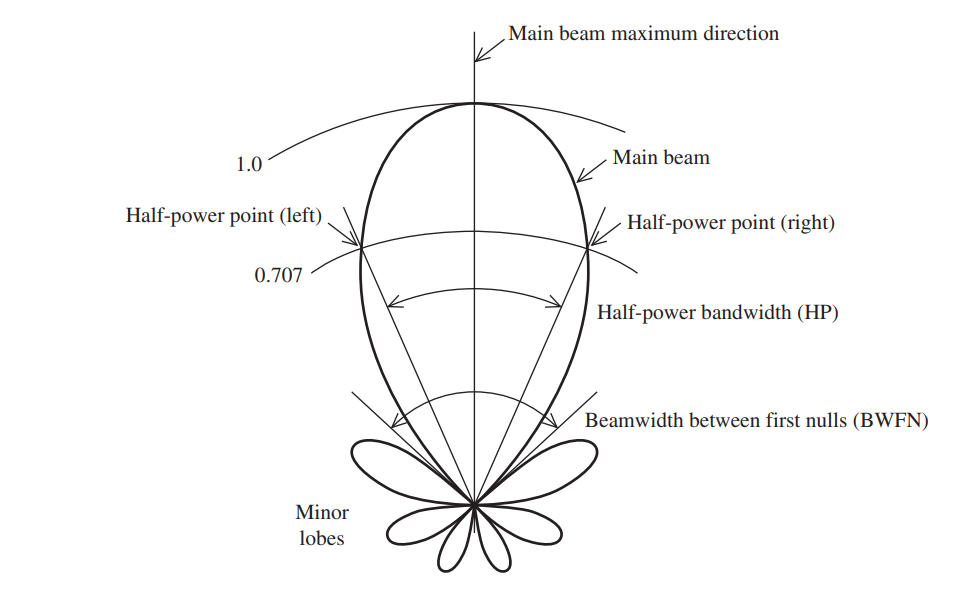
\includegraphics[width = 11cm]{img/patern1.png}
    \caption{Parámetros del patrón de radiación para una antena con características directivas. \cite{stutzman2012antenna}.}
    \label{fig:patern}
\end{figure}

La figura \ref{fig:patern}, muestra un patrón de radiación de una antena directiva, donde se pueden observar los lóbulos laterales y el haz principal. El haz principal es la dirección de máxima radiación, mientras que los lóbulos laterales son las direcciones de radiación secundarias.\\

El haz principal se define en términos de potencia y se conoce como HPBW o Haz de Media Potencia. El HPBW es el ángulo entre los puntos de la curva de radiación que tienen la mitad de la potencia máxima, es decir donde se ve una disminución de 3 dB.\\

\subsection{Directividad}

\subsection{Ganancia}

\subsection{Polarización}

\subsection{Ancho de banda}

\subsection{Perdidas y eficiencia}

\paragraph{Impedancia de entrada}

\paragraph{Perdidas de espacio libre}

\paragraph{Perdidas de superficie}

\paragraph{Perdidas de cable}


\section{Antenas de apertura}

\subsection{Antenas parabólicas}

\paragraph{Foco primario}

\paragraph{Cassegrain}

\paragraph{Gregorian}

\paragraph{Off-axis}

\section{Antenas de alimentación}

\subsection{Tipos de antenas de alimentación}

\paragraph{Yagi-Uda}

\paragraph{Bocina}

\paragraph{Log-Periódica}

\paragraph{Antenas de semiespacio}

\paragraph{Antenas de parche}

\section{Receptores heterodinos}

\subsection{¿Qué es un receptor heterodino?}

\subsection{Radio definida por software}

\subsection{Transformada Rápida de Fourier}


\section{Radiotelescopios}

\subsection{¿Qué es un radiotelescopio?}

\subsection{Línea de Hidrógeno Neutro}

\subsection{CHARTS y FRB}










\section{Conceptos previos}
\subsection{Radiotelescopio}

En la astronomía clásica, se utilizan telescopios que operan en el rango visible del espectro electromagnético, el mismo rango que tiene el ojo humano, donde estos actúan como el receptor o, al mismo tiempo, una cámara fotográfica. En contraste, un radiotelescopio es un instrumento que observa en longitudes de onda mucho más grandes en el espectro de radio. Estos telescopios, usualmente, son constituidos por un reflector parabólico que concentra la luz obtenida en su foco, donde se ubica un receptor de radio.\\

Un telescopio de radio tiene consideraciones distintas a uno óptico, ya que el anterior puede observar con múltiples receptores a la vez como lo es el caso de una cámara fotográfica, pero uno de radio, debe tener un receptor de mayor envergadura proporcional con el tamaño de la longitud de onda, lo que limita el número de receptores a uno en la gran mayoría de los casos.\\

Otro punto importante a destacar, es la característica de ciencia que se puede realizar con estos telescopios, ya que para el caso de la línea de Hidrógeno, se pueden observar fuentes que no necesariamente provienen de estrellas o, para frecuencias más bajas, estrellas con que irradian fuera del rango visible.

\subsection{Línea de Hidrógeno Neutro}

El movimiento de un electrón en un átomo de Hidrógeno neutro, genera un campo magnético que se acopla con los espines del protón y el electrón. \quotes{Este acople da cuenta de la radiación a 1420 MHz que viene de la transición entre dos niveles energéticos de primer nivel del estado fundamental del hidrógeno} \cite{Restrepo2023}.\\

Observar H1 permite estudiar la evolución del universo primitivo, rescatando información proveniente de la transición de la \quotes{Época Oscura} a la formación de las primeras fuentes de luminosas del universo.

\subsection{CHARTS y FRB}

Los fenómenos astrofísicos transitorios de radio o FRB, son eventos de extremadamente corta duración y origen desconocido que ocurren en un amplio rango de frecuencias. Estos pulsos inspiraron el proyecto CHARTS, para apoyar su búsqueda y estudio.\\

El proyecto CHARTS, es una colaboración entre la Universidad de Chile y la Universidad de Toronto con el objetivo de construir un arreglo de 128 sintonizadas para operar en el rango de 300MHz a 500MHz en el marco de la búsqueda de FRB.

\subsection{Polarización}

La polarización de una antena hace referencia a la polarización del campo eléctrico y magnético que produce al irradiar potencia al medio. Convencionalmente, se utilizan 2 polarizaciones para las observaciones astronómicas y para las telecomunicaciones, la polarización lineal y la polarización circular.\\

\begin{figure}
    \centering
    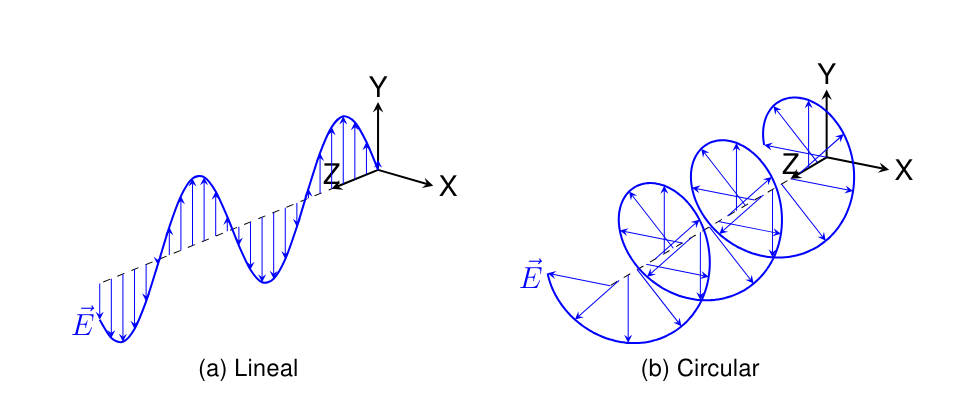
\includegraphics[width = 15cm]{img/pol.png}
    \caption{A la izquierda se tiene una polarización lineal del campo electromagnético y a la derecha una polarización circular izquierda\cite{Astudillo2014}.}
    \label{fig:pol}
\end{figure}

La polarización linear, se genera con el campo eléctrico contenido en un plano, como se puede ver en la figura \ref{fig:pol}. En contraste, la polarización circular se produce en un caso particular cuando el campo eléctrico rota con una frecuencia constante en torno a un eje y su magnitud es constante. De lo contrario, se produce una polarización elíptica en torno al eje de propagación, tal como se observa en la figura anterior.\\

Las distintas polarizaciones, se pueden generar por medios constructivos en la geometría de la antena o medios de alteración de fase, ya sea por efectos de largo eléctrico o modulaciones electrónicas para generar el desfase de las líneas alimentadoras.

\subsection{Antenas de Apertura}

Las antenas de apertura son aquellas que su funcionamiento es caracterizado por el campo generado en una superficie reflectante, la cual se denomina como apertura. Dentro de las antenas de apertura están las antenas de apertura parabólica que utilizan una superficie parabólica para irradiar potencia. Existen 4 tipos de configuraciones para las antenas parabólicas, \textit{Cassegrain}, \textit{Gregorian}, \textit{off-axis} o fuera de foco y \textit{axial feed} o Foco Primario. Esta última es el que se utilizará para el proyecto.\\

Estas antenas concentran la radiación en un punto focal dependiendo de su geometría de paraboloide. Usualmente, se instala la antena alimentadora en el foco de la parábola o en el foco de la segunda parábola para las antenas \textit{Cassegrain} y \textit{Gregorian}.\\

\begin{figure}
    \centering
    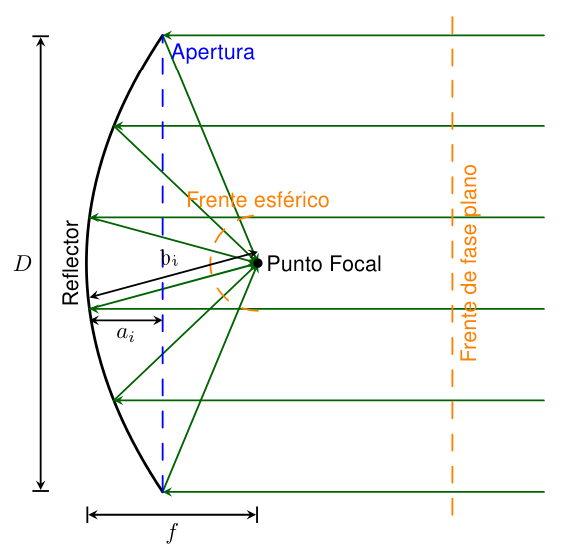
\includegraphics[width = 10cm]{img/parabola.png}
    \caption{Geometría característica de un reflector parabólico para el tipo de Foco Primario\cite{Astudillo2014}.}
    \label{fig:parabola}
\end{figure}

La representación de seguimiento de rayos en dos dimensiones para un reflector parabólico en la figura \ref{fig:parabola}, hace referencia al tipo de configuración a utilizar en la construcción del reflector del nuevo radio telescopio.


\subsection{Antena Alimentadora}

La antena alimentadora, es aquella antena que captura la radiación proveniente de los reflectores. Se debe ocupar una antena con un patrón de radiación directivo, con el objetivo de captar la mayor cantidad de la luz concentrada por el reflector.\\

Ejemplos de antenas directivas:

\begin{itemize}
    \item Yagi-Uda
    \item Bocina
    \item Log-Periódica
    \item Antenas de semi espacio
    \item Antenas de parche
\end{itemize}

\subsection{Receptor Heterodino}

Los receptores heterodinos, o coherentes, son los más usados en la radioastronomía. Su función característica es convertir una señal de alta frecuencia a un rango de menor frecuencia, conservando la información de fase y de amplitud para poder ser digitalizada con facilidad\cite{Finger2013}. Para esto, los receptores utilizan un mezclador con un oscilador local para adquirir la señal desde la antena alimentadora para luego ser procesada digitalmente.\\

\begin{figure}
    \centering
    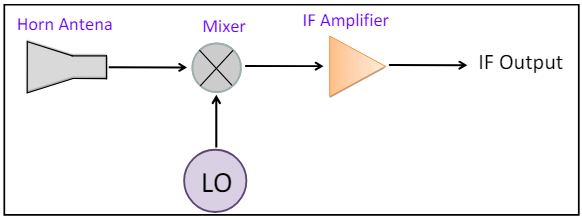
\includegraphics[width = 10cm]{img/heterodine.png}
    \caption{Diagrama de bloques de un receptor heterodino para astronomía de tipo DSB.}
    \label{fig:radio}
\end{figure}

La figura \ref{fig:radio} corresponde a un diagrama de bloques de la configuracion más simple para un receptor heterodino. Contiene una antena receptora, un mezclador de radio frecuencia, un oscilador local y un amplificador de bajo ruido.

\section{Estado del Arte}

El estado del arte para radiotelescopios, en particular de radios telescopios de reflectores con diámetros de 3 metros o menos. En este caso, la principal línea de desarrollo es en la radio-interferometría y el uso de sistemas de bajo ruido, a la vez que la disminución de los costos para nuevos instrumentos.\\

Los esfuerzos para la búsqueda de FRB y, específicamente, en la detección del origen de estos pulsos de alta energía, puede lograrse con el uso de \textit{Pathfinding} al correlacionar 2 telescopios separados por largas distancias para hacer interferometría de línea de base muy larga, o VLBI por su sigla en inglés (T. A. Cassanelli, 2021). Experimento que se quiere hacer con el proyecto CHARTS y este nuevo telescopio.\\

Luego, en el contexto de la construcción un nuevo radiotelescopio para observar la línea de 21cm, se tienen los siguientes exponentes que implementan diversas técnicas que inspiran el desarrollo y operación que se desea con el telescopio CPT.\\


\subsection{Telescopio Mini}

\begin{figure}
    \centering
    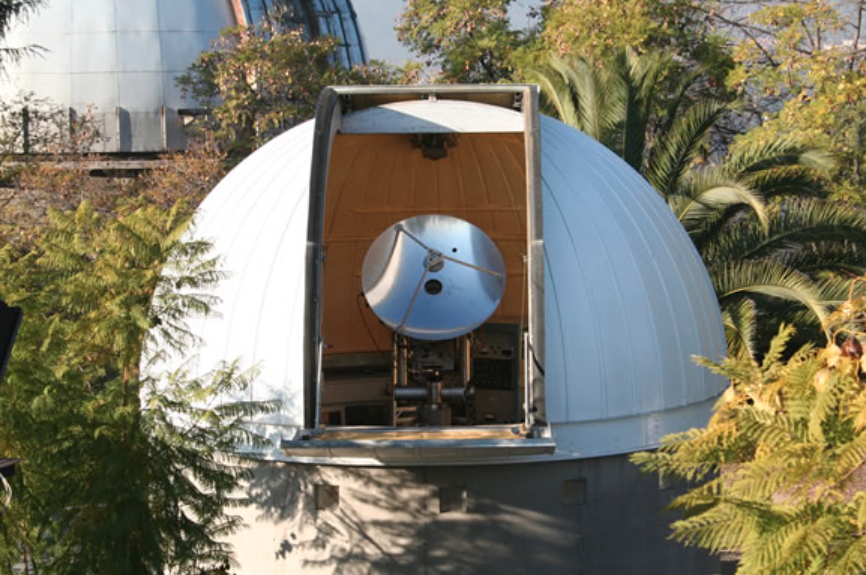
\includegraphics[width = 12cm]{img/mini.png}
    \caption{Telescopio MINI en el Observatorio Cerro Calan de la Facultad de Ciencia Físicas y Matemáticas de la Universidad de Chile\cite{DAS2024}}
    \label{fig:mini}
\end{figure}

El telescopio de la figura \ref{fig:mini}, se encuentra en el cerro Calán, a pocos metros de la ubicación de los cimientos para, CPT, ejemplificando las consideraciones de operar en un ambiente extremadamente saturado de interferencia de radiofrecuencia que se puede encontrar en el centro de la ciudad principal del país como Santiago.

\subsection{Telescopio FAST}

\begin{figure}
    \centering
    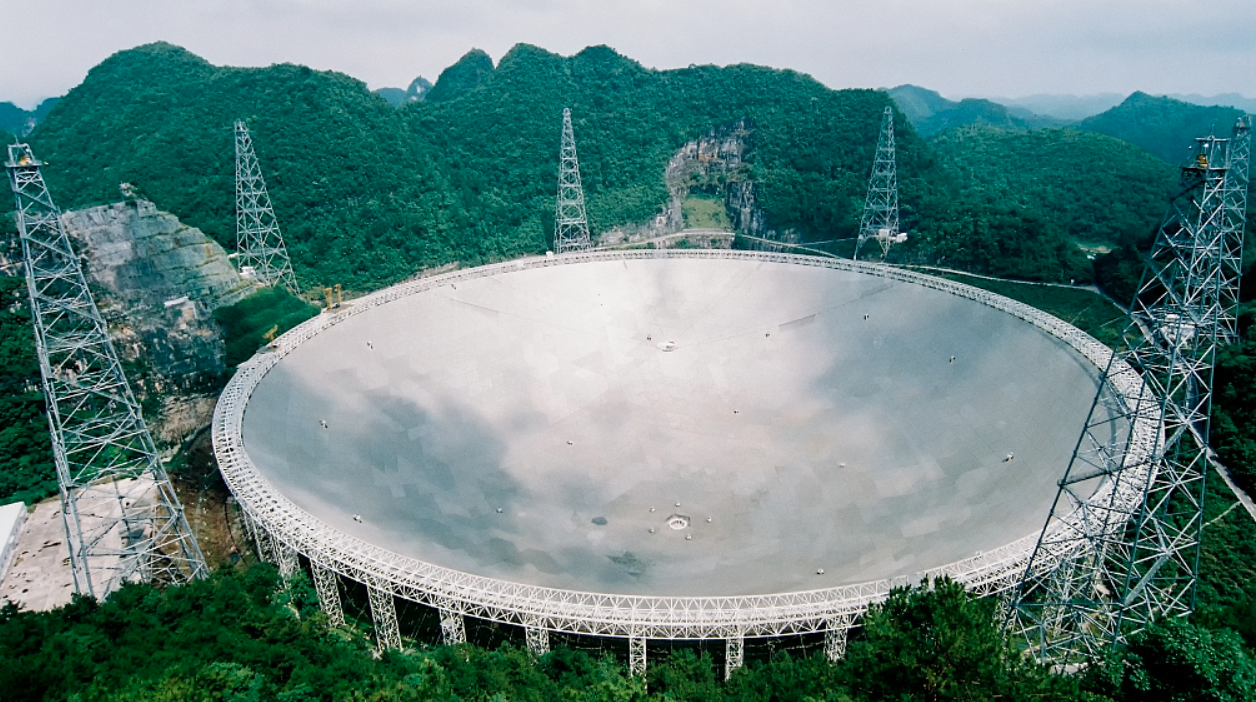
\includegraphics[width = 12cm]{img/fast.png}
    \caption{Telescopio Fast en la provincia de Guizhou, China \cite{FAST2024}.}
    \label{fig:fast}
\end{figure}

La figura \ref{fig:fast}, corresponde a un telescopio de 500 metros de apertura con un alimentador posicionado en el foco de la superficie parabólica primaria que puede hacer observaciones de la linea de 21cm y de FRB. El cual se ubica en China, en la provincia de Guizhou.

\subsection{Telescopio SRT}

\begin{figure}
    \centering
    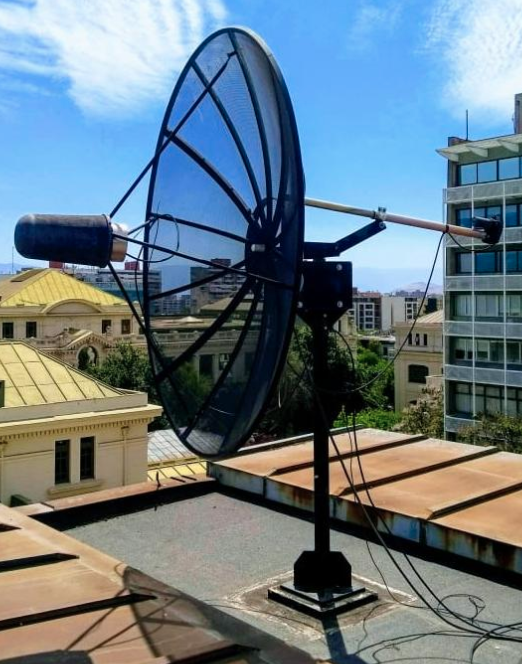
\includegraphics[width = 6cm]{img/srt.png}
    \caption{Telescopio SRT del MIT en la azotea del departamento de ingeniería eléctrica de la FCFM\cite{Curotto2019}.}
    \label{fig:srt}
\end{figure}

El Telescopio de la figura \ref{fig:srt}, se encuentra ubicado en la azotea del edificio del Departamento Ingeniería Eléctrica de la Universidad de Chile, equipado con receptores y filtros diseñados para observar la línea de Hidrógeno neutro. El material de sus reflectores es similar al que se utilizará en CPT.

\subsection{Observatorio CHIME}

\begin{figure}
    \centering
    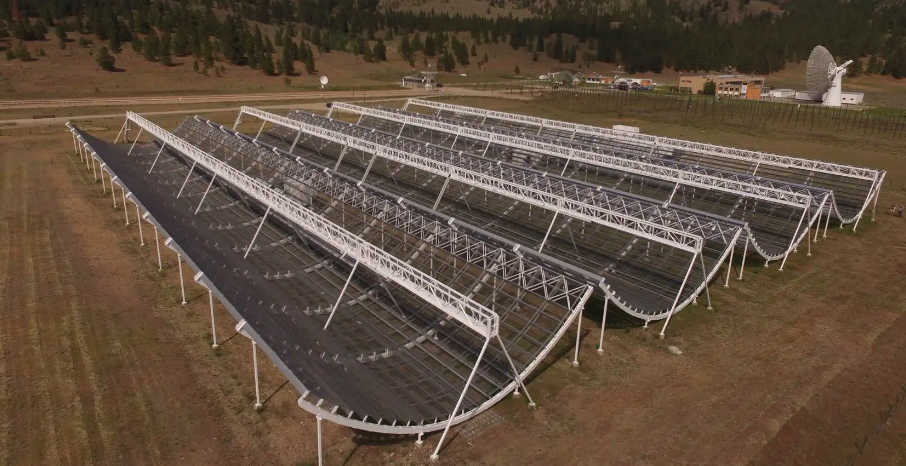
\includegraphics[width = 12cm]{img/chime.png}
    \caption{Telescopio experimental CHIME en Canada \cite{CHIME}.}
    \label{fig:chime}
\end{figure}

La figura \ref{fig:chime}, corresponde al telescopio experimental sin partes móviles, sintonizado para observar Hidrógeno y con un correlacionador capaz generar una apertura sintética para encontrar fenómenos astrofísicos transitorios de radio. Trabaja con una arquitectura de instrumentos remotos.

\subsection{Guía de Construcción de Radiotelescopio con una RTL-SDR}

Un enfoque para hacer radioastronomía con componentes comerciales y de bajo costo. Se utilizan radios definidas por software como receptor de radiofrecuencia y destaca las herramientas y software para observar la línea de 21cm.

\begin{figure}
    \centering
    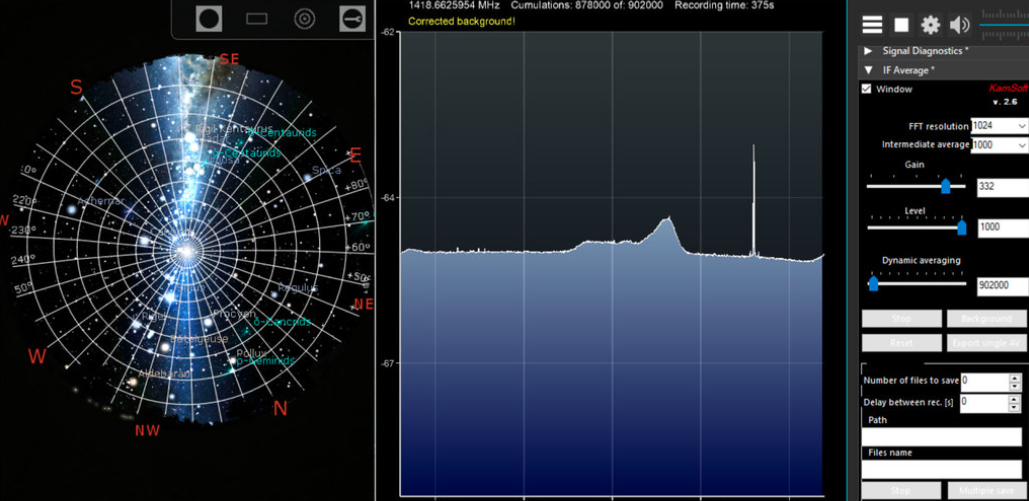
\includegraphics[width = 12cm]{img/rtlsdr.png}
    \caption{Software utilizado por RTL-SDR Blog para observar Hidrógeno neutro con una RTL-SDR\cite{RTLSDR2018}.}
    \label{fig:rtl}
\end{figure}

La figura \ref{fig:rtl}, corresponde al software de recepción de radio sintonizado en la frecuencia de emisión del hidrógeno neutro a la derecha, además del software de seguimiento astronómico y catalogo de objetos de interés.